%% Based on a TeXnicCenter-Template by Gyorgy SZEIDL.
%%%%%%%%%%%%%%%%%%%%%%%%%%%%%%%%%%%%%%%%%%%%%%%%%%%%%%%%%%%%%

%------------------------------------------------------------
%
\documentclass{article}
\usepackage{amsmath}%
\usepackage{amsfonts}%
\usepackage{amssymb}%
\usepackage{graphicx}
%--------------------------------------------------------
\begin{document}
\title{Notes on Real-time Ambient Occlusion with screen space ray-casting}
\author{Ugo Varetto}
\date{October 12, 2009}

\maketitle

\begin{abstract}
\noindent This document describes a technique to perform real-time screen space ambient occlusion
through ray-casting in screen-space with adaptive re-computation of integration radius
and interactive control over integration radius and integration step size.
\end{abstract}


%%%%%%%%%%%%%%%%%%%%%%%%%%%%%%%%%%%%%%%%%%%
\section{Introduction}

Ambient occlusion for a point is a measure of how much such point is hidden by
its surrounding environment: the higher the occlusion value, the less amount of
ambient light will hit the point. Attempts have been made to give a mathematical
description of ambient occlusion, the first mathematical formalization
of something similar to ambient occlusion I know about is contained in \cite{Zhukov et al. 1998}.

Ambient occlusion is a cheap way of approximating global illumination effects used
to give a photo-realistic appearance to synthetically generated images. Note that global
illumination techniques are not just useful to produce nice looking images
but are also a way to make a viewer understand the actual spatial shape of objects (Fig.
 \ref{aoandnoao}).

\begin{figure}[!ht]
\caption{Molecule rendering with and without ambient occlusion}
\begin{center}
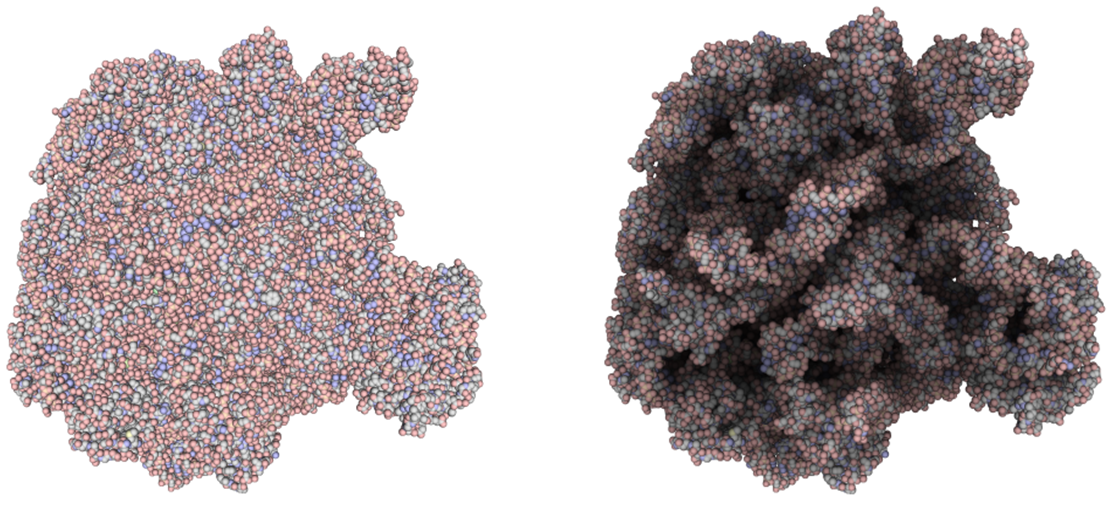
\includegraphics[width=12cm]{images/AO_AND_NOAO.png}
\end{center}
\label{aoandnoao}
\end{figure}

%REMOVED 
%Also techniques used to compute ambient occlusion can actually be applied in 
%gradient spaces and any $k$-dimensional space to analyze various properties of surfaces,
%polytopes and even (directed) point clouds (which will all be the subject of my own future research).  

Techniques smilar to the ones used to compute ambient occlusion 
can be adapted to approximate radiance transfer and generate color-bleeding effects in screen space.

Different methods for computing ambient occlusion have been presented over the
past years; most of them fall into one of two categories: 

\begin{enumerate}
	\item per-vertex or per-face ambient occlusion pre-computation
	\item real-time per-pixel computation
\end{enumerate}

Vertex based pre-computation methods are fine for static geometry with a high polygon
count while per-pixel techniques work well for dynamic scenes, do not require the input
to be a set of polygons, and therefore integrate well with ray-tracing and volume rendering. 

The method described in this article is a per-pixel technique which was implemented
between 2007 and 2008 as an add-on to a real-time ray-tracer for large molecular models
and further modified to work with any type of data.
The key technique employed by the algorithm is to use the angular coefficient of rays
to select the points that contribute to the overall occlusion.
 

%%%%%%%%%%%%%%%%%%%%%%%%%%%%%%%%%%%%%%%%%%%%%  
\section{Screen Space Ambient Occlusion}

Screen space ambient occlusion for a pixel $p$ can be approximated by 
computing the average of occlusion contributions coming from a number of directions:

\begin{equation}
%%% Ap = 1/N * Sum(i = 1..N, Api)
%%% Api = 1 / S * Sum( j = 1..N, Apij )
A_{p} = \frac{1}{N}\sum_{i=1}^N A_{pi}
\label{ssao}
\end{equation}

Where $A_{p}$ is the total occlusion at $p(x,y)$ and $A_{pi}$ is the contribution 
coming from direction $i$ to the total occlusion.

\begin{figure}[!ht]
\caption{Depth map profile along ray}
\begin{center}
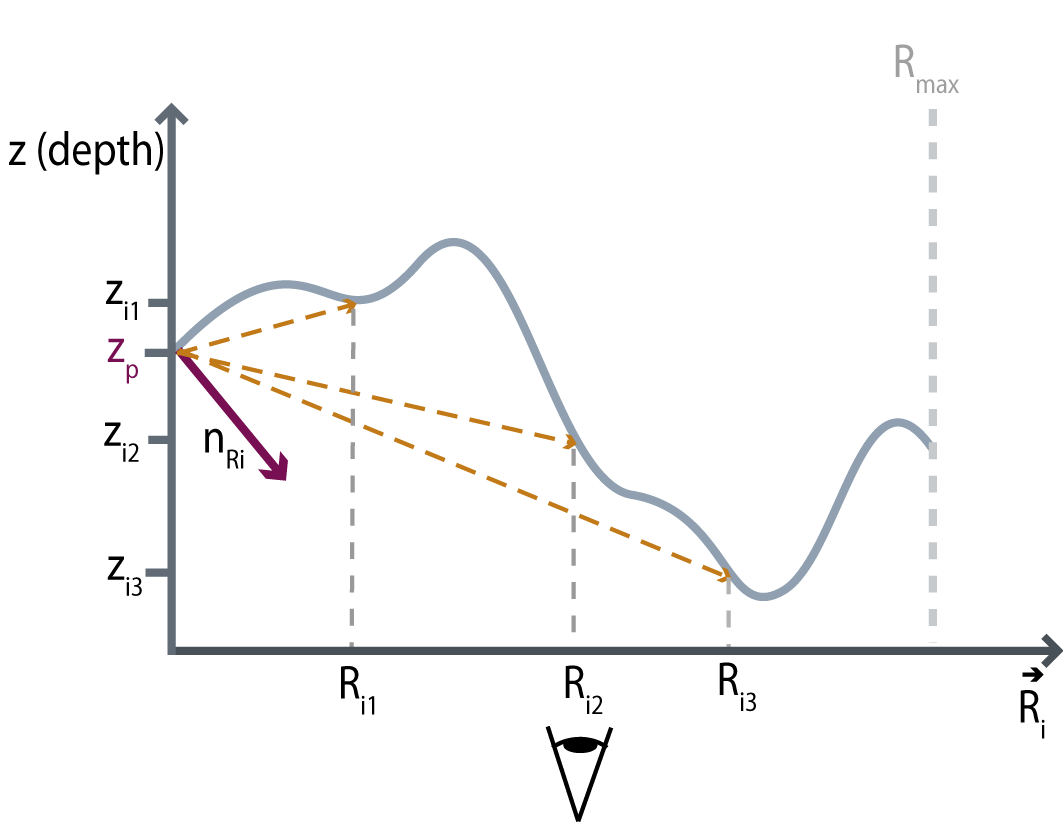
\includegraphics{images/SSAO-screenspace.png}
\end{center}
\label{ssaocreenspace}
\end{figure}

The term $A_{pi}$ is computed by integrating the ambient occlusion along a linear path
in screen space:

\begin{equation}
A_{pi} = \frac{1}{S}\sum_{j=1}^Socc(\vec{p},\vec{o}_{ij})
\label{ssaoray}
\end{equation}

Where:
\begin{itemize}
	\item $S$ is the total number of steps
	\item $\vec{p}$ and $\vec{o}$ are $3D$\footnote{ 2D pixel coordinates + 1D depth coordinate} screen coordinates
	\item $occ(\vec{a}, \vec{b})$ is the contribution from point $\vec{b}$ to the occlusion
	      of point $\vec{a}$ 
\end{itemize}

The contribution to the total occlusion of a point in screen space from another point in 
screen space is approximated by first transforming the two points into world space then applying the 
formula:
\begin{equation}
occ(\vec{p},\vec{o}) = \frac{max\left( 0, \hat{N}_{P} \cdot \frac{\vec{O}-\vec{P}}{\left|\vec{O} - \vec{P}\right|}\right)}
                            {f\left( \left|\vec{O} - \vec{P}\right|\right)}
\label{occ}
\end{equation}                                 

Where:
\begin{itemize}
	\item $\vec{O}$ and $\vec{P}$ are the world space coordinates of $\vec{o}$ and $\vec{p}$
	\item $\hat{N}$ is the unit normal in world coordinates at point $\vec{P}$
	\item $f(d)$ is a (usually polynomial) function of the distance $d$ between the two points 
\end{itemize}

Note that several variations are possible here: the normal at $\vec{O}$ can be used instead of 
$\frac{\vec{O}-\vec{P}}{\left|\vec{O} - \vec{P}\right|}$;
all the computation can be carried on in screen space; the normals can be precomputed or computed on the fly
from the tangent space.

Also it is possible to use a varying-step approach where the step increases with the distance (e.g. $step(d)=kd^2$) to take into account high spatial frequencies only at close distance; this allows to take into account contributions from both near and far fragments while still running at reasonable frame rates.

$f(d)$ can be e.g.:
\begin{equation}
f(d) = B(d_{max})d^2 + 1
\end{equation}
Where $B(d_{max})$ is a coefficient dependent on the maximum ray length. The value assigned to $B$ ensures that
$occ(\vec{p}, \vec{o}_{d_{max}})$ is always equal to a predefined occlusion value.  

%%%%%%%%%%%%%%%%%%%%%%%%%%%%%%%%%%%%%%%%%%%%%  
\section{Algorithm}

According to the equations defined in the previous sections ambient occlusion at each pixel can be
computed by selecting a number of directions in $2D$ screen space and averaging the occlusion contributions
along each direction.

\begin{figure}[!ht]
\caption{Rays in screen space}
\begin{center}
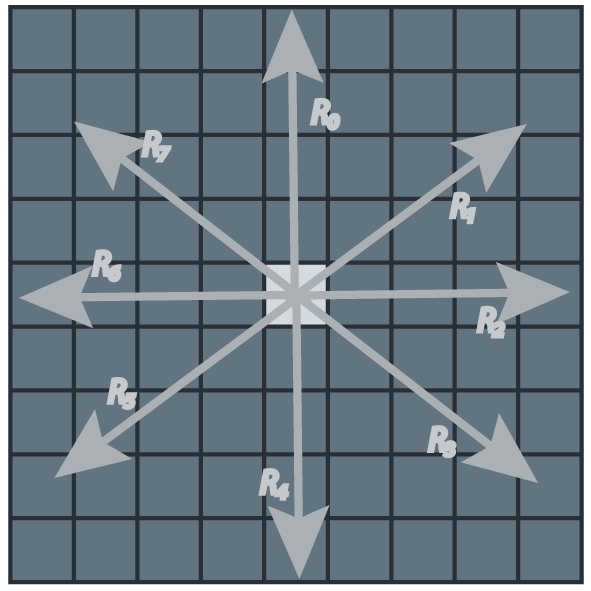
\includegraphics{images/SSAO-rays.png}
\end{center}
\label{ssaorays}
\end{figure}
The occlusion along a specific direction is computed by averaging the contributions of each point found along
the $2D$ ray shot in that direction; now, in order to minimize the number of times Eq.\eqref{occ} is applied we need to
understand if a point along the ray is at all visible from the ray starting point (the pixel being shaded) i.e. if a line connecting
the two points does not intersect any geometry. It turns out this is quite easy to understand by comparing 
the angular coefficient of the $3D$\footnotemark[\value{footnote}]
line connecting the ray starting point with the previous intersection point and
the one of the $3D$\footnotemark[\value{footnote}] line connecting the current point with the ray staring point.

The algorithm to compute the per-pixel occlusion is therefore:

\begin{enumerate}
\item \textit{FOR EACH} pixel $\vec{p}$ select directions in $2D$ screen coordinates
\item \textit{FOR EACH} direction follow a linear path up to \texttt{MAX\_LENGTH} in that direction and
\item \textit{FOR EACH} $2D$ point $\vec{o}$ along the path compute the angular coefficient
      $c = \frac{\left(z_{p} - z_{o}\right)}{\left|\vec{o} - \vec{p}\right|}$ where
      $z_{o}$ and $z_{p}$ are the depths of pixels $\vec{o}$ and $\vec{p}$ 
\item \textit{IF} the newly computed coefficient is greater than the previously computed one
      \textit{THEN} replace the previously computed coefficient with the new one and add the contribution
      of the current point to the total occlusion by applying Eq.\eqref{occ}
\end{enumerate}


\begin{figure}[!ht]
\caption{Angular coefficient along ray}
\begin{center}
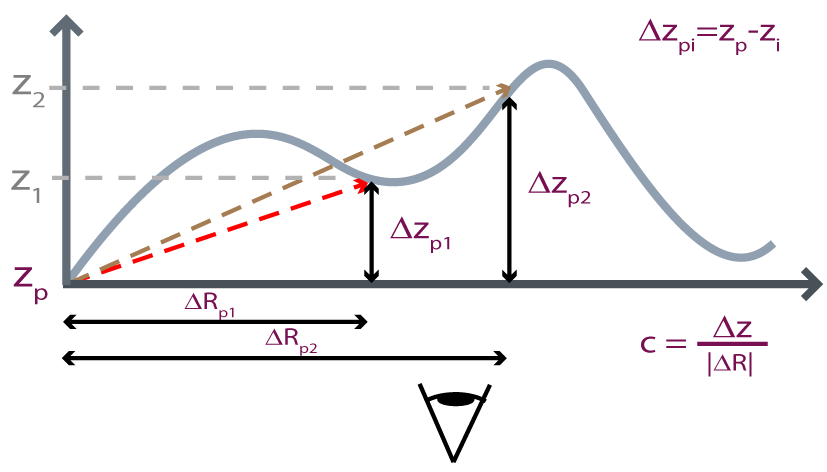
\includegraphics{images/SSAO-angularcoeff.png}
\end{center}
\label{ssaoangularcoeff}
\end{figure}

The \texttt{MAX\_LENGTH} length of the ray in pixels is a percentage of the object/scene bounding sphere radius projected into screen space.
In cases where the scene completely fills the view it is actually easier to use a percentage of the view size. 

Note that the value $\left(z_{p} - z_{o}\right)$ is negative for points $\vec{o}$ that are farther away 
from then viewer than point $\vec{p}$.

\section{Real-time rendering technique} 

The data needed by the algorithm described in the previous section are:

\begin{itemize}
	\item depth information for the entire scene
	\item world space coordinates of each fragment (pixel)
	\item normalized world space normals of each fragment (pixel) 
\end{itemize}

which can all be computed in a single pre-rendering step by using OpenGL's multiple-render-target feature.

Real-time ambient occlusion computation is therefore performed in two separate rendering stages:

\begin{enumerate}
	\item store pixel world positions, normals and depths in texture targets
	\item compute per-pixel ambient occlusion (and shade) from stored data 
\end{enumerate}

See Figure ~\ref{ssaoadiagram} on page ~\pageref{ssaoadiagram}.

\begin{figure}[!ht]
\caption{Rendering stages}
\begin{center}
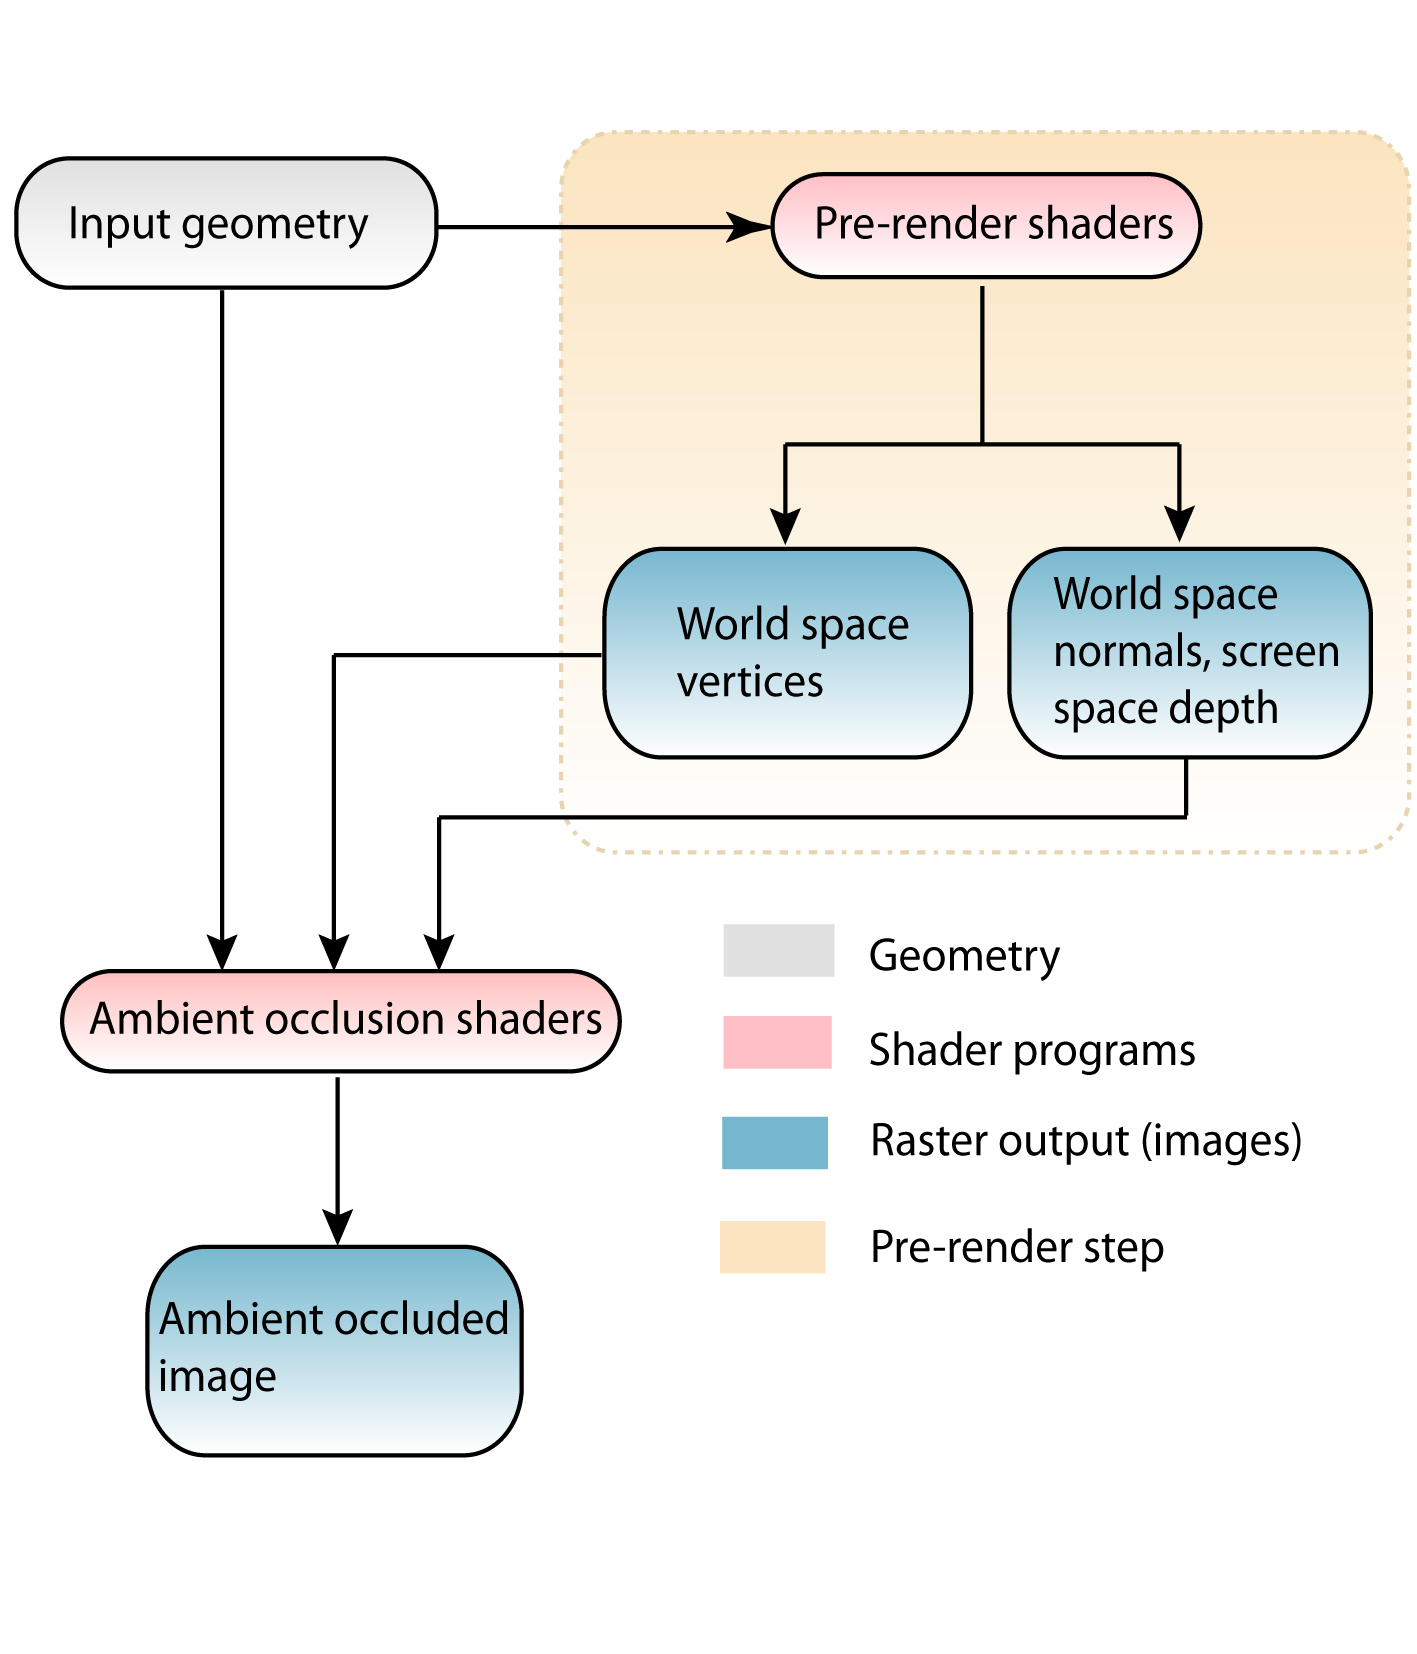
\includegraphics{images/SSAO-diagram.png}
\end{center}
\label{ssaoadiagram}
\end{figure}

%%%%%%%%%%%%%%%%%%%%%%%%%%%%%%%%%%%%%%%%%%%%%  
\section{Conclusion and future directions}

Screen space ambient occlusion can be successfully used to approximate global illumination effects, depending 
on the intended usage it might however show serious limitations, the biggest of which is the inability to take
into account objects which lay outside the current view frustum; techniques can be applied to
mitigate this problem such as using a different (bigger) frustum for the pre-rendering stage or implementing methods similar to reflection mapping.
Note however that the ability to use only the visible geometry for performing ambient occlusion computation can indeed
be desirable in cases where the viewpoint is actually inside the model to explore as it is the case for architectural
walkthroughs, interior designs or scientific visualization in general. 

The plan is to use the described technique to perform radiance-transfer like behavior in a new volume/ray-casting
based rendering engine currently in development. The basic idea is to implement a  multi-stage algorithm
where the first stage takes care of illuminating objects visible from light sources and the subsequent stages to compute
ambient light from previously illuminated geometry.

Also I plan to extend a previously developed ambient occlusion generation application with a variation of this
algorithm to generate pre-computed cube and spherical ambient occlusion maps.  

%%%%%%%%%%%%%%%%%%%%%%%%%%%%%%%%%%%%%%%%%%%%%  
\begin{thebibliography}{9}

\bibitem {BavoilSainz2009} Bavoil L. and Sainz M.
\textit{Multi-Layer Dual-Resolution Screen-Space Ambient Occlusion},
ACM SIGGRAPH 2009 Talk Program.

\bibitem {Ritschel} T. Ritschel, T. Grosch and H. P. Seidel,
\textit{Approximating Dynamic Global Illumination in Image Space}, MPI Informatik
                                                                                             
\bibitem {Sainz} Sainz, M.,
\textit{Real-Time Depth Buffer Based Ambient Occlusion}, 
Game Developer Conference 2008, San Francisco.

\bibitem {ShanmugamArikan2007} Perumaal Shanmugam and Okan Arikan,
\textit{Hardware accelerated ambient occlusion techniques on GPUs},
Proceedings of the 2007 symposium on Interactive 3D graphics and games, Seattle.  

\bibitem {TatarchukGDC2006} Tatarchuk N.
\textit{Parallax Occlusion Mapping for Highly Detailed Surface Rendering},
Game Developer Conference 2006, San Francisco.

\bibitem {Kontkanen2005i3d} Kontkanen J. and Laine S. 
\textit{Ambient Occlusion Fields}, 
Proceedings of ACM SIGGRAPH 2005 Symposium on Interactive 3D Graphics and Games,
Pages 41--48, 2005 ACM Press.

\bibitem {Zhukov et al. 1998} Zhukov S., Iones A., Kronin G. 
\textit{An ambient light illumination model}, Rendering techniques '98:
proceedings of the Eurographics Workshop, Vienna - AT, 1998.

\end{thebibliography}

%%%%%%%%%%%%%%%%%%%%%%%%%%%%%%%%%%%%%%%%%%%%%  
\end{document}
%%%%%%%%%%%%%%%%%%%%%%%%%%%%%%%%%%%%%%%%%%%%%  

